\chapter{Other matching methods}

\section{Fisher--Paterson}

For text $T=\texttt{gcatatatgccggata}$ and pattern $P=\texttt{cata}$ perform Fisher--Patterson algorithm.

$T_a=(0,0,1,0,1,0,1,0,0,0,0,0,0,1,0,1)$, $P_a=(0,1,0,1)$\\
$T_c=(0,1,0,0,0,0,0,0,0,1,1,0,0,0,0,0)$, $P_c=(1,0,0,0)$\\
$T_g=(1,0,0,0,0,0,0,0,1,0,0,1,1,0,0,0)$, $P_g=(0,0,0,0)$\\
$T_t=(0,0,0,1,0,1,0,1,0,0,0,0,0,0,1,0)$, $P_t=(0,0,1,0)$\medskip\\
$T_a \times {P_a}^R = (0,0,1,0,2,0,2,0,1,0,0,0,0,1,0,2,0,1,0)$\\
$T_c \times {P_c}^R = (0,0,0,0,1,0,0,0,0,0,0,0,1,1,0,0,0,0,0)$\\
$T_g \times {P_g}^R = (0,0,0,0,0,0,0,0,0,0,0,0,0,0,0,0,0,0,0)$\\
$T_t \times {P_t}^R = (0,0,0,0,1,0,1,0,1,0,0,0,0,0,0,1,0,0,0)$\medskip\\
$R = (0,0,1,0,4,0,3,0,2,0,0,0,1,2,0,3,0,1,0)$

Each position in $R$ represents a number of matched characters when $R$ is aligned with string $T$, $|R| = |T|+ |P| - 1$, so it contains also partial matches.

\section{Rank \& Select}

\clearpage
\section{Wavelet Tree}

\begin{figure}
\tikzstyle{level 1}=[level distance=1.5cm, sibling distance=8cm]
\tikzstyle{level 2}=[level distance=1.5cm, sibling distance=4cm]
\tikzstyle{level 3}=[level distance=1.5cm, sibling distance=4cm]
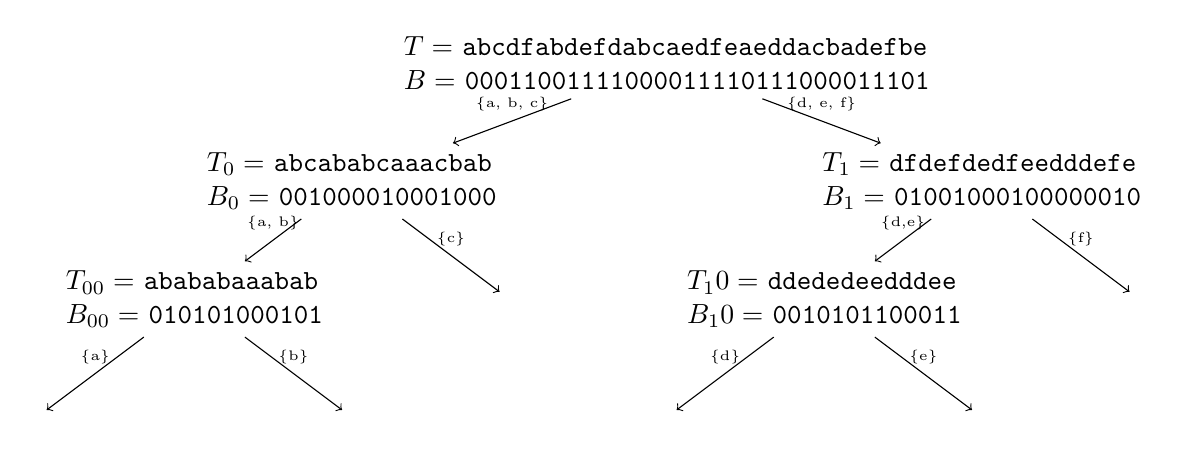
\begin{tikzpicture}[grow=down]
	\node[align=left] {
	 	$T=$ \texttt{abcdfabdefdabcaedfeaeddacbadefbe}\\
		\red$B=$ \texttt{00011001111000011110111000011101}
  }
	child {
		node[align=left] {
			$T_0=$ \texttt{abcababcaaacbab}\\
			\red$B_0=$ \texttt{001000010001000}
		}
		child {
			node[align=left] {
				$T_{00}=$ \texttt{abababaaabab}\\
				\red$B_{00}=$ \texttt{010101000101}
			}
			child {
        node{\texttt{}}
        edge from parent [->] node [midway,above] {\tiny \{a\}}
      }
			child {
        node{\texttt{}}
        edge from parent [->] node [midway,above] {\tiny \{b\}}
      }
      edge from parent [->] node [midway,above] {\tiny \{a, b\}}
		}
		child {
      node{\texttt{}}
      edge from parent [->] node [midway,above] {\tiny \{c\}}
    }
    edge from parent [->] node [midway,above] {\tiny \{a, b, c\}}
	}
	child {
		node[align=left] {
			$T_1=$ \texttt{dfdefdedfeedddefe}\\
			\red$B_1=$ \texttt{01001000100000010}
		}
		child {
			node[align=left]{
				$T_10=$ \texttt{ddededeedddee}\\
				\red$B_10=$ \texttt{0010101100011}
			}
			child {
        node{\texttt{}}
        edge from parent [->] node [midway,above] {\tiny \{d\}}
      }
			child {
        node{\texttt{}}
        edge from parent [->] node [midway,above] {\tiny \{e\}}
      }
      edge from parent [->] node [midway,above] {\tiny \{d,e\}}
		}
		child {
      node{\texttt{}}
      edge from parent [->] node [midway,above] {\tiny \{f\}}
    }
    edge from parent [->] node [midway,above] {\tiny \{d, e, f\}}
	};
\end{tikzpicture}
\caption{Wavelet tree for string $T$=abcdfabdefdabcaedfeaeddacbadefbe.}
\end{figure}

$\mathrm{rank}_T(\texttt{b}, 10) = \mathrm{rank}_{B_{00}}(1, \mathrm{rank}_{B_0}(0, \mathrm{rank}_B(0, 10)))$\\
$\mathrm{select}_T(\texttt{d}, 5) = \mathrm{select}_B(1, \mathrm{select}_{B_1}(0, \mathrm{select}_{B_{10}}(0, 5)))$

Support rank, select and symbol on posstion queris.

\section{Compressed Suffix Array}
